\chapter{Methodology}
\label{chap:Methodology}
This research will be divided into two consecutive phases.

The first part, \typenameref{subsec:DataCollectionAndParsing}, will focus on retrieving the pricing-data on a predetermined set of routes. This phase will gather data during a period of 6~weeks and parse it into a new interlinked format. The information retrieved and parsed during this period will be used as the census for the whole study.

The second phase, \typenameref{subsec:OptionValuationModels}, will deal with the analysis of the data and build simulation models. These simulation models will be used to test the performance of the different configurations of option seller and customer. Furthermore, they will provide answers to the research questions as defined in \todo{ref}.

A more detailed description of the first phase will be given in the next section. The thorough definition of the simulation models used in this study will be given in \ref{chap:ModelDevelopment}.


\section{Data collection and parsing}
\label{subsec:DataCollectionAndParsing}
In the first phase information on flights will be collected from the Internet. This data will be used as the census for this study. The price setting systems, simulation models and prediction system will all be based upon this dataset.

The website of \href{http://google.nl/flights}{Google Flights} will be used to gather this information. I have selected this resource, because contrary to intermediary sites like Expedia.com, Google Flights does show the lowest available fare and merely redirect users to the airliner's site. Furthermore, direct calls to Google's RPC-server enable users to request XSS-protected JSON-arrays with flight data. See \autoref{app:DataExtractedFromGoogleFlightsRPCRequest} for a detailed list of information included in these arrays.

In this research I will restrict myself to collecting data on 22~different round-trip flights. Of these 22~routes, 10~flights cover domestic routes within the United~States, 6 are domestic routes within the European Union, and the remaining 6~routes are international. The 10~US domestic flights are two routes selected from the 5~busiest domestic airports within the US, as retrieved from the \citeA{bts13}. The 6~EU domestic flights are a selection of routes between the airports \emph{AMS}, \emph{CDG}, \emph{MAD}, and \emph{LHR}. These four~airports are amongst the top~5 busiest airports in Europe \citeA{eur13}. Due to Google Flight's limitation of only providing data for flights departing from the US and the EU, I have selected 6~international routes departing from those areas. See \autoref{app:SelectedRoutes} for the detailed list of selected routes. The routes examined in this study are all round-trip flights with an interval of 7~days between the departure date for the outbound and inbound flight.

\begin{figure*}
\centering
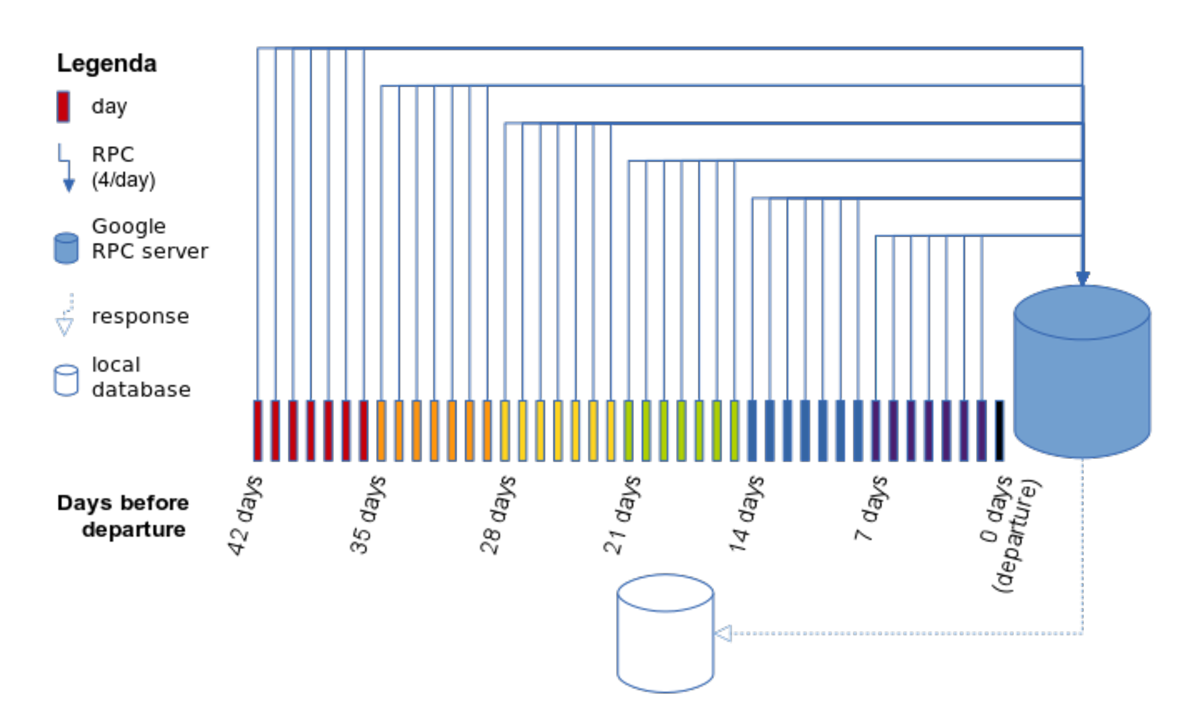
\includegraphics[width=0.8\textwidth]{figures/DataRetrievalProcess}
\caption{Data retrieval process}
\label{fig:DataRetrievalProcess}
\end{figure*}

Data will be collected on the previously mentioned routes departing during the period from Monday the $20^{th}$ of August up until Sunday the $30^{th}$ of September. Price data on all these flights will start 6~weeks prior to departure, up until the day before take-off. The data retrieval can best be illustrated with the help of \autoref{fig:DataRetrievalProcess}. Each day (represented by a rectangular box) an automated program will send a \emph{Remote Procedure Call} (blue arrow) to the \emph{RPC-server} of Google Flights (blue cylinder). This request asks the server to send data on a flight that meets certain specifications. For example, the first call the program makes on July the $9^{th}$ (6~weeks prior to start of collection of specific route) is ``\emph{return data on all flights from ATL to MCO departing on August $20^{th}$ and returning on August $27^{th}$ (7 days after departure)}''. The call is send to the server as a JSON-formatted request (See \autoref{app:SampleJSONRPC} for an example). In return, Google's server will send data on all the flights that meet those requirements (blue dashed arrow) and the automated program will store the received information in a local database (white cylinder). The next day the same process is repeated by sending the exact same query to the RPC-server again. This procedure is repeated each day up until the day before departure.

The goal of this data collection phase is to track fare changes on flights for every day up to 42~days before departure. Because Google Flights does not always send back data on the same flights, the same RPC is send every 6~hours (at 00:00, 06:00, 12:00 and 18:00) \footnote{Each blue arrow thus represents 4 requests on that single day}. This methodology thus enforces reliability of the data collection, as there is a much higher probability the airfare for a specific flight will be returned in one of these requests. However, it also creates 4~price observations spread over 4~time windows for each day before departure. These multiple price observations will thus have to be converted into a single data point.

To do so, each flight will be distinguished using the characteristics described in \autoref{subsec:FlightTicket}, and departure times will be converted to UTC\@. Next, the time window $p_{t_n}$ of the lookup time relative to the actual departure time is determined for each flight, where $n = \lfloor \frac{\scriptstyle{hours\ before\ departure}}{6} \rfloor + 1$. Because files are downloaded for 4~times per day, they can be assigned to time windows consisting of 6~hours. For example, an airfare retrieved 33 hours before departure of the flight will be assigned to time window $p_{t_6}$, where $6 = \lfloor \frac{33}{6} \rfloor + 1$. Because ticket prices will be acquired from 1~day up until 42~days before departure, a total of 168~time windows will be available for each flight, ranging from $p_{t_5}$ till $p_{t_{172}}$.

After parsing of the files, the prices of the 6~hour time windows will be converted to represent daily values. This is done by aggregating every 4~time windows into a single airfare by averaging the values. For instance, the time windows $p_{t_{17}}$, $p_{t_{18}}$, $p_{t_{19}}$ and $p_{t_{20}}$ will be averaged into a single value $p_{d_4}$ representing the ticket price for that specific flight as available 4~days before departure. An illustration of this process is given in \autoref{fig:conversionOfTimeslotsIntoDailyAirfares}.

\begin{figure}
    $$
    \kbordermatrix{
                   &\multispan4\hfill$\scriptstyle 1\,dbd$\hfill    &        \\
            \omit  &\multispan4\quad\downbracefill\quad             &        \\
            \#1    & p_{t_5} & p_{t_6} & p_{t_7} & p_{t_8} & \vrule & \cdots \\
            \#2    & p_{t_5} & p_{t_6} & p_{t_7} & p_{t_8} & \vrule & \cdots \\
            \vdots & \vdots  & \vdots  & \vdots  & \vdots  & \vrule & \ddots \\
            \#n    & p_{t_5} & p_{t_6} & p_{t_7} & p_{t_8} & \vrule & \cdots
    }
    \Rightarrow
    \kbordermatrix{
                   & 1\,\scriptstyle{dbd}       & \cdots & 42\,\scriptstyle{dbd}              \\
            \#1    & \overline{p_{t_{5,6,7,8}}} & \cdots & \overline{p_{t_{169,170,171,172}}} \\
            \#2    & \overline{p_{t_{5,6,7,8}}} & \cdots & \overline{p_{t_{169,170,171,172}}} \\
            \vdots & \vdots                     & \ddots & \vdots                             \\
            \#n    & \overline{p_{t_{5,6,7,8}}} & \cdots & \overline{p_{t_{169,170,171,172}}}
    }
    $$
    \caption{Conversion of time windows into daily airfares}
    \label{fig:conversionOfTimeslotsIntoDailyAirfares}
\end{figure}

When certain timeslots contain no price observation, this single timeslot is left out of the calculation of the average airfare for that specific number of days before departure. Only when all 4~of the timeslots for a specific day have no data available, the value in the new data matrix is assigned as \emph{missing value} (i.e. n/a).

The whole illustrated process only describes one route (i.e. \emph{ATL} to \emph{MCO}) departing on one specific date (i.e. departure on \emph{August $20^{th}$}). The automated program however takes into account every route described in \autoref{app:selectedroutes}, and all dates in the period from August $20^{th}$ till September $30^{th}$.

After retrieval of the flight information, the data is parsed and stored in the \href{http://www.hdfgroup.org/HDF5/}{HDF5-format}. This data format is often used in big data analysis, and enables quick reading of big sets of data to memory. Following the loading into RAM, the data will be converted to a \href{http://pandas.pydata.org/}{Pandas} object after which analysis can be done.

Distinction between flights is made by hashing flight's  properties\footnote{The \emph{call sign} of each segment and \emph{ticketing code} of the flight}. Prices of the flight will be stored in the HDF5-file using the hash as the identification key. This enables easy extraction of price fluctuations within exact same flights relative to time. The time of departure of each flight is converted to UTC.

For illustration, an example extract from the HDF5-data matrix containing the first few flights of the route AMS-JFK can be seen in \autoref{fig:extractFromAMStoJFK} of \autoref{chap:DataAnalysis}.

